% Lammle, ch. 11
\chapter{VLANs and inter-VLAN routing}
\label{chap:lammle-ch11}

I know I keep telling you this, but so you never forget it, here I go, one last time: By default, switches break up collision domains and routers break up broadcast domains.
Okay, I feel better! Now we can move on.

In contrast to the networks of yesterday that were based on collapsed
backbones, today's network design is characterized by a flatter
architecture -- thanks to switches. So now what? How do we break up
broadcast domains in a pure switched internetwork? By creating virtual
local area networks (VLANs). A VLAN is a logical grouping of network
users and resources connected to administratively defined ports on a
switch. When you create VLANs, you'regiven the ability to create smaller
broadcast domains within a layer~2 switched internetwork by assigning
different ports on the switch to service different subnetworks. A VLAN
is treated like its own subnet or broadcast domain, meaning that frames
broadcast onto the network are only switched between the ports logically
grouped within the same VLAN.

So, does this mean we no longer need routers? Maybe yes; maybe no. It
really depends on what your particular networking needs and goals are.
By default, hosts in a specific VLAN can't communicate with hosts that
are members of another VLAN, so if you want inter-VLAN communication,
the answer is that you still need a router or inter-VLAN routing (IVR).

In this chapter, you're going to comprehensively learn exactly what a VLAN is and how VLAN memberships are used in a switched network.
You'll also become well-versed in what a trunk link is and how to configure and verify them.

I'll finish this chapter by demonstrating how you can make inter-VLAN communication happen by introducing a router into a switched network.
Of course, we'll configure our familiar switched network layout we used in the last chapter for creating VLANs and for implementing trunking and Inter-VLAN routing on a layer~3 switch by creating switched virtual interfaces (SVIs).


\section{VLAN basics}

\Cref{fig:flat-network-structure} illustrates the flat network architecture that used to be so typical for layer~2 switched networks.
With this configuration, every broadcast packet transmitted is seen by every device on the network regardless of whether the device needs to receive that data or not.


\begin{figure}
   \centering
   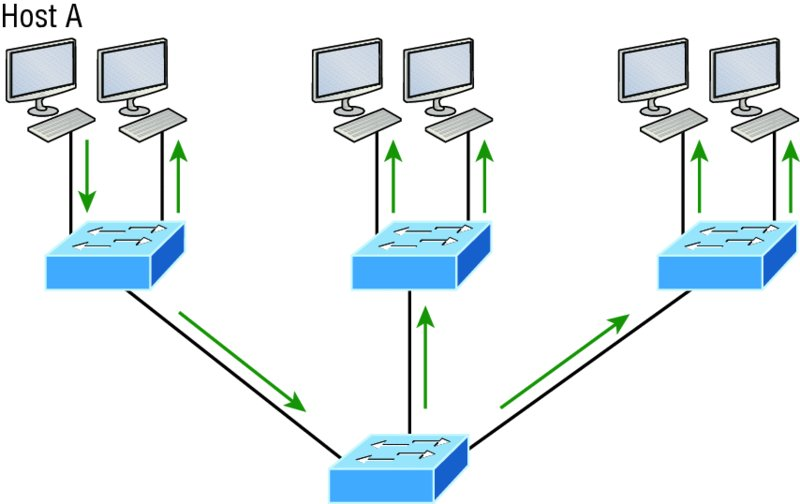
\includegraphics{images/c11f001.jpg}
   \caption{Flat network structure}
   \label{fig:flat-network-structure}
\end{figure}


By default, routers allow broadcasts to occur only within the originating network, while switches forward broadcasts to all segments.
Oh, and by the way, the reason it's called a \emph{flat network} is because it's one \emph{broadcast domain}, not because the actual design is physically flat.
In \cref{fig:flat-network-structure} we see Host A sending out a broadcast and all ports on all switches forwarding it -- all except the port that originally received it.

Now check out \cref{fig:benefit-switched-network}.
It pictures a switched network and shows Host A sending a frame with Host D as its destination.
Clearly, the important factor here is that the frame is only forwarded out the port where Host D is located.


\begin{figure}
   \centering
   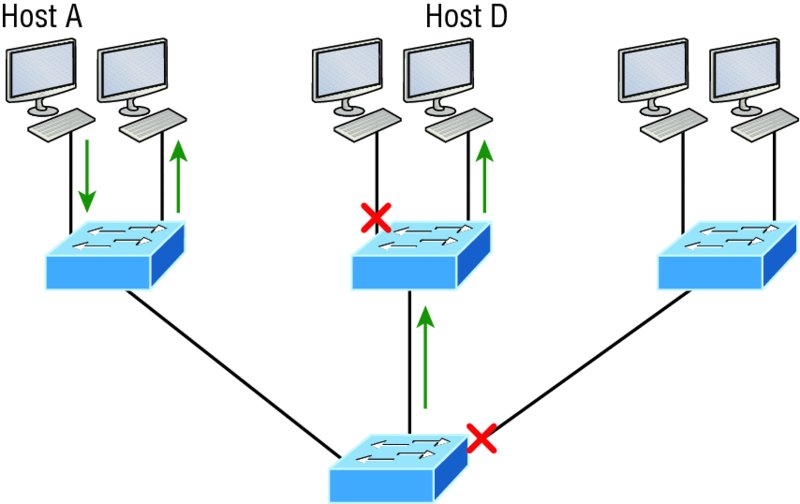
\includegraphics{images/c11f002.jpg}
   \caption{The benefit of a switched network}
   \label{fig:benefit-switched-network}
\end{figure}


This is a huge improvement over the old hub networks, unless having one
\emph{collision domain} by default is what you really want for some
reason!

Okay -- you already know that the biggest benefit gained by having a layer~2 switched network is that it creates individual collision domain
segments for each device plugged into each port on the switch. This
scenario frees us from the old Ethernet density constraints and makes us
able to build larger networks. But too often, each new advance comes
with new issues. For instance, the more users and devices that populate
and use a network, the more broadcasts and packets each switch must
handle.

And there's another
big issue -- security! This one is real trouble because within the
typical layer~2 switched internetwork, all users can see all devices by
default. And you can't stop devices from broadcasting, plus you can't
stop users from trying to respond to broadcasts. This means your
security options are dismally limited to placing passwords on your
servers and other devices.

But wait -- there's hope if you create a \emph{virtual} LAN (VLAN)!
You can solve many of the problems associated with layer~2 switching with VLANs, as you'll soon see.

VLANs work like this: \cref{fig:one-switch-one-lan} shows all hosts in this very small company connected to one switch, meaning all hosts will receive all frames, which is the default behavior of all switches.

\begin{figure}
   \centering
   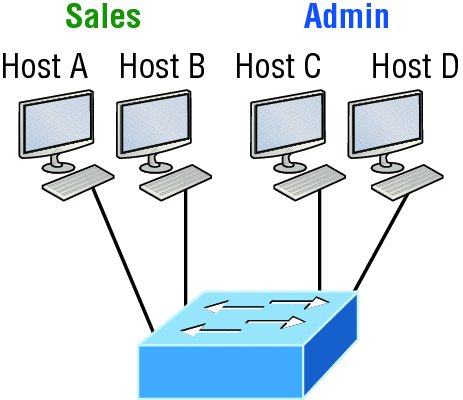
\includegraphics{images/c11f003.jpg}
   \caption[One switch, one LAN]{One switch, one LAN: Before VLANs, there were no separations between hosts.}
   \label{fig:one-switch-one-lan}
\end{figure}

If we want to separate the host's data, we could either buy another
switch or create virtual LANs, as shown in \cref{fig:one-switch-two-lan}.

\begin{figure}
   \centering
   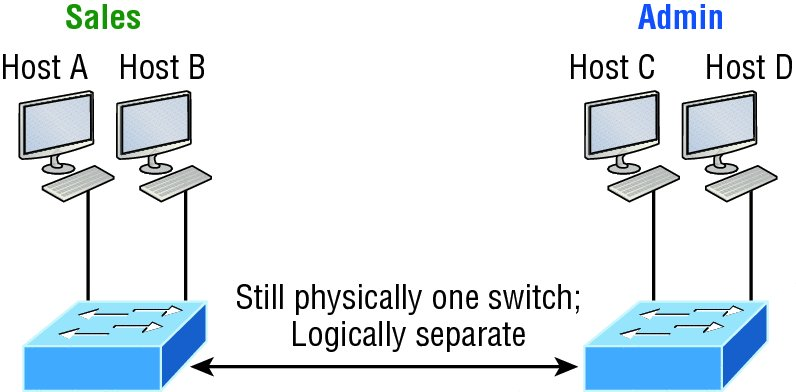
\includegraphics{images/c11f004.jpg}
   \caption[One switch, two virtual LANs]{One switch, two virtual LANs (\emph{logical} separation between hosts): still physically one switch, but this switch acts as many separate devices.}
   \label{fig:one-switch-two-lan}
\end{figure}

In \cref{fig:one-switch-two-lan}, I configured the switch to be two separate LANs, two subnets, two broadcast domains, two VLANs -- they all mean the same thing -- without buying another switch.
We can do this 1,000 times on most Cisco switches, which saves thousands of dollars and more!

Notice that even though the separation is virtual and the hosts are all still connected to the same switch, the LANs can't send data to each other by default.
This is because they are still separate networks, but no worries -- we'll get into inter-VLAN communication later in this chapter.

Here's a short list of ways VLANs simplify network management:

\begin{enumerate}
   \item
      Network adds, moves, and changes are achieved with ease by just configuring a port into the appropriate VLAN.
   \item
      A group of users that need an unusually high level of security can be put into its own VLAN so that users outside of that VLAN can't communicate with the group's users.
   \item
   As a logical grouping of users by function, VLANs can be considered independent from their physical or geographic locations.
   \item
   VLANs greatly enhance network security if implemented correctly.
   \item
   VLANs increase the number of broadcast domains while decreasing their size.
\end{enumerate}

Coming up, we'll thoroughly explore the world of switching, and you learn exactly how and why switches provide us with much better network services than hubs can in our networks today.



\subsection{Broadcast control}

Broadcasts occur in every protocol, but how often they occur depends upon three things:

\begin{enumerate}
   \item
      The type of protocol
   \item
      The application(s) running on the internetwork
   \item
      How these services are used
\end{enumerate}

Some older applications have been rewritten to reduce their bandwidth
consumption, but there's a new generation of applications that are so
bandwidth greedy they'll consume any and all they can find. These
gluttons are the legion of multimedia applications that use both
broadcasts and multicasts extensively. As if they weren't enough
trouble, factors like faulty equipment, inadequate segmentation, and
poorly designed firewalls can seriously compound the problems already
caused by these broadcast-intensive applications. All of this has added
a major new dimension to network design and presents a bunch of new
challenges for an administrator. Positively making sure your network is
properly segmented so you can quickly isolate a single segment's
problems to prevent them from propagating throughout your entire
internetwork is now imperative. And the most effective way to do that is
through strategic switching and routing!

Since switches have become more affordable, most everyone has replaced
their flat hub networks with pure switched network and VLAN
environments. All devices within a VLAN are members of the same
broadcast domain and receive all broadcasts relevant to it. By default,
these broadcasts are filtered from all ports on a switch that aren't
members of the same
VLAN. This is great because you get all the benefits you would with a
switched design without getting hit with all the problems you'd have if
all your users were in the same broadcast domain -- sweet!

\subsection{Security}

But there's always a catch, right? Time to get back to those security
issues. A flat internetwork's security used to be tackled by connecting
hubs and switches together with routers. So it was basically the
router's job to maintain security. This arrangement was pretty
ineffective for several reasons. First, anyone connecting to the
physical network could access the network resources located on that
particular physical LAN. Second, all anyone had to do to observe any and
all traffic traversing that network was to simply plug a network
analyzer into the hub. And similar to that last, scary, fact, users
could easily join a workgroup by just plugging their workstations into
the existing hub. That's about as secure as a barrel of honey in a bear
enclosure!

But that's exactly what makes VLANs so cool. If you build them and
create multiple broadcast groups, you can still have total control over
each port and user! So the days when anyone could just plug their
workstations into any switch port and gain access to network resources
are history because now you get to control each port and any resources
it can access.

And that's not even all -- VLANs can be created in harmony with a
specific user's need for the network resources. Plus, switches can be
configured to inform a network management station about unauthorized
access to those vital network resources. And if you need inter-VLAN
communication, you can implement restrictions on a router to make sure
this all happens securely. You can also place restrictions on hardware
addresses, protocols, and applications. \emph{Now} we're talking
security -- our honey barrel is now sealed tightly, made of solid
titanium and wrapped in razor wire!

\subsection{Flexibility and scalability}

If you've been paying attention so far, you know that layer~2 switches only read frames for filtering because they don't look at the Network layer protocol.
You also know that by default, switches forward broadcasts to all ports. But if you create and implement VLANs, you're essentially creating smaller broadcast domains at layer~2.

As a result, broadcasts sent out from a node in one VLAN won't be
forwarded to ports configured to belong to a different VLAN. But if we
assign switch ports or users to VLAN groups on a switch or on a group of
connected switches, we gain the flexibility to exclusively add only the
users we want to let into that broadcast domain regardless of their
physical location. This setup can also work to block broadcast storms
caused by a faulty network interface card (NIC) as well as prevent an
intermediate device from propagating broadcast storms throughout the
entire internetwork. Those evils can still happen on the VLAN where the
problem originated, but the disease will be fully contained in that one
ailing VLAN!

Another advantage is that when a VLAN gets too big, you can simply create more VLANs to keep
the broadcasts from consuming too much bandwidth. The fewer users in a
VLAN, the fewer users affected by broadcasts. This is all good, but you
seriously need to keep network services in mind and understand how the
users connect to these services when creating a VLAN. A good strategy is
to try to keep all services, except for the email and Internet access
that everyone needs, local to all users whenever possible.

\section{Identifying VLANs}

Switch ports are layer~2-only interfaces that are associated with a physical port that can belong to only one VLAN if it's an access port or all VLANs if it's a trunk port.

Switches are definitely pretty busy devices.
As myriad frames are switched throughout the network, switches have to be able to keep track of all of them, plus understand what to do with them depending on their associated hardware addresses.
And remember -- frames are handled differently according to the type of link they're traversing.

There are two different types of ports in a switched environment.
Let's take a look at the first type in \cref{fig:access-ports}.

\begin{figure}
   \centering
   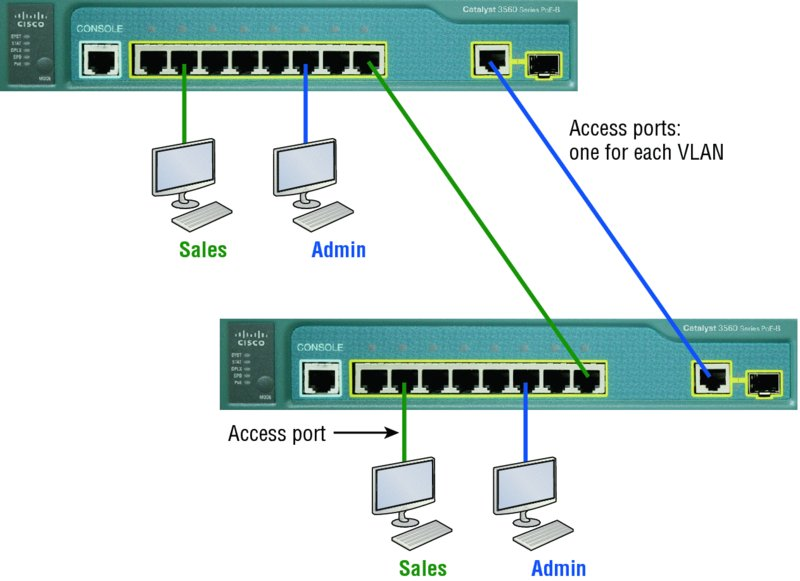
\includegraphics{images/c11f005.jpg}
   \caption{Access ports}
   \label{fig:access-ports}
\end{figure}

Notice there are access ports for each host and an access port between switches -- one for each VLAN.

\paragraph{Access ports}
An \emph{access port} belongs to and carries the traffic of only one VLAN.
Traffic is both received and sent in native formats with no VLAN information (tagging) whatsoever.
Anything arriving on an access port is simply assumed to belong to the VLAN assigned to the port.
Because an access port doesn't look at the source address, tagged traffic -- a frame with added VLAN information -- can be correctly forwarded and received only on trunk ports.

With an access link, this can be referred to as the \emph{configure VLAN} of the port.
Any device attached to an \emph{access link} is unaware of a VLAN membership -- the device just assumes it's part of some
broadcast domain.
But it doesn't have the big picture, so it doesn't understand the physical network topology at all.

Another good bit of information to know is that switches remove any VLAN
information from the frame before it's forwarded out to an access-link
device. Remember that access-link devices can't communicate with devices
outside their VLAN unless the packet is routed. Also, you can only
create a switch port to be either an access port or a trunk port -- not
both. So you've got to choose one or the other and know that if you make
it an access port, that port can be assigned to one VLAN only. In
\protect\hyperlink{c11.xhtmlux5cux23figure11-5}{Figure 11.5}, only the
hosts in the Sales VLAN can talk to other hosts in the same VLAN. This
is the same with the Admin VLAN, and they can both communicate to hosts
on the other switch because of an access link for each VLAN configured
between switches.

\paragraph{Voice access ports}
Not to confuse you, but all that I just said about the fact that an access port can be assigned to only one VLAN is really only sort of true.
Nowadays, most switches will allow you to add a second VLAN to an access port on a switch port for your voice traffic,
called the voice VLAN. The voice VLAN used to be called the auxiliary
VLAN, which allowed it to be overlaid on top of the data VLAN, enabling
both types of traffic to travel through the same port. Even though this
is technically considered to be a different type of link, it's still
just an access port that can be configured for both data and voice
VLANs. This allows you to connect both a phone and a PC device to one
switch port but still have each device in a separate VLAN.

\paragraph{Trunk ports}
Believe it or not, the term \emph{trunk port}%
\footnote{HP uses the term \emph{trunk port} to refer to an EtherChannel (\vref{sec:etherchannel}) and uses the term \emph{tagged ports} to refer to Cisco's trunk ports.}
was inspired by the telephone system trunks, which carry multiple telephone conversations at a time.
So it follows that trunk ports can similarly carry multiple VLANs at a time as well.

A \emph{trunk link} is a 100, 1,000, or 10,000 Mbps point-to-point link between two switches, between a switch and router, or even between a switch and server, and it carries the traffic of multiple VLANs -- from~1 to 4094 VLANs at a time.
But the amount is really only up to 1001 unless you're going with something called extended VLANs.

Instead of an access link for each VLAN between switches, we'll create a trunk link, demonstrated in \cref{fig:trunk-links}.

\begin{figure}
   \centering
   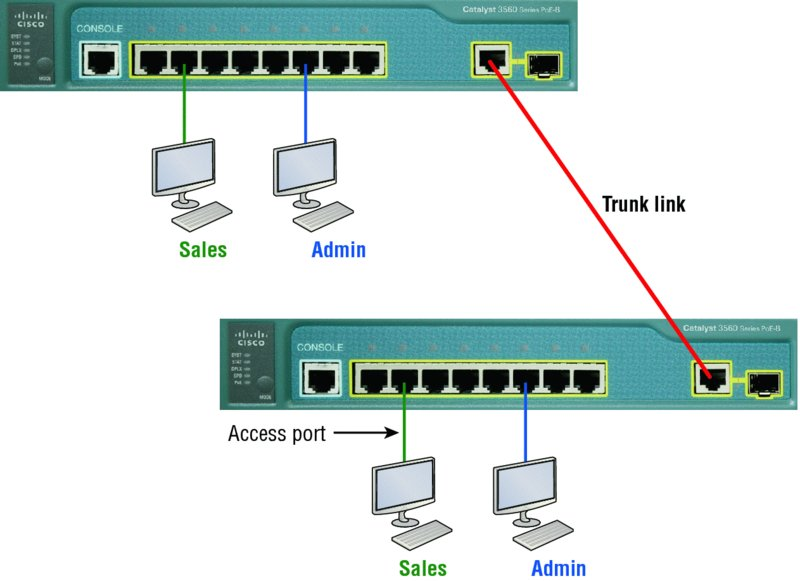
\includegraphics{images/c11f006.jpg}
   \caption{VLANs can span across multiple switches by using trunk links, which carry traffic for multiple VLANs}
   \label{fig:trunk-links}
\end{figure}

Trunking can be a real advantage because with it, you get to make a
single port part of a whole bunch of different VLANs at the same time.
This is a great feature because you can actually set ports up to have a
server in two separate broadcast domains simultaneously so your users
won't have to cross a layer~3 device (router) to log in and access it.
Another benefit to trunking comes into play when you're connecting
switches. Trunk links can carry the frames of various VLANs across them,
but by default, if the links between your switches aren't trunked, only
information from the configured access VLAN will be switched across that
link.

It's also good to know that all VLANs send information on a trunked link
unless you clear each VLAN by hand, and no worries, I'll show you how to
clear individual VLANs from a trunk in a bit.

Okay -- it's finally time to tell you about frame tagging and the VLAN identification methods used in it across our trunk links.

\subsection{Frame tagging}

As you now know, you can set up your VLANs to span more than one connected switch.
You can see that going on in \cref{fig:trunk-links}, which depicts hosts from two VLANs spread across two switches.
This flexible, power-packed capability is probably the main advantage to implementing VLANs, and we can do this with up to a thousand VLANs and thousands upon thousands of hosts!

All this can get kind of complicated -- even for a switch -- so there needs to be a way for each one to keep track of all the users and frames as they travel the switch fabric and VLANs.
When I say, ``switch fabric,'' I'm just referring to a group of switches that share the same VLAN information.
And this just happens to be where \emph{frame tagging} enters the scene.
This frame identification method uniquely assigns a user-defined VLAN ID to each frame.

Here's how it works: Once within the switch fabric, each switch that the
frame reaches must first identify the VLAN ID from the frame tag. It
then finds out what to do with the frame by looking at the information
in what's known as the filter table. If the frame reaches a switch that
has another trunked link, the frame will be forwarded out of the
trunk-link port.

Once the frame reaches an exit that's determined by the forward/filter
table to be an access link matching the frame's VLAN ID, the switch will
remove the VLAN identifier. This is so the destination device can
receive the frames without being required to understand their VLAN
identification information.

Another great thing about trunk ports is that they'll support tagged and
untagged traffic simultaneously if you're using 802.1q trunking, which
we will talk about next. The trunk port is assigned a default port VLAN
ID (PVID) for a VLAN upon which all untagged traffic will travel. This
VLAN is also called the native VLAN and is always VLAN 1 by default, but
it can be changed to any VLAN number.

Similarly, any untagged or tagged traffic with a NULL (unassigned) VLAN
ID is assumed to belong to the VLAN with the port default PVID. Again,
this would be VLAN 1 by default. A packet with a VLAN ID equal to the
outgoing port native VLAN is sent untagged and can communicate to only
hosts or devices in that same VLAN. All other VLAN traffic has to be
sent with a VLAN tag to communicate within a particular VLAN that
corresponds with that tag.



\subsection{VLAN identification methods}

VLAN identification is what switches use to keep track of all those
frames as they're traversing a switch fabric. It's how switches identify
which frames belong to which VLANs, and there's more than one trunking
method.

\subsubsection{Inter-switch link (ISL)}

\emph{Inter-Switch Link (ISL)} is a way of explicitly tagging VLAN
information onto an Ethernet frame. This tagging information allows
VLANs to be multiplexed over a trunk link through an external
encapsulation method. This allows the switch to identify the VLAN
membership of a frame received over the trunked link.

By running ISL, you can interconnect multiple switches and still
maintain VLAN information as traffic travels between switches on trunk
links. ISL functions at layer~2 by encapsulating a data frame with a new
header and by performing a new cyclic redundancy check (CRC).

Of note is that ISL is proprietary to Cisco switches and is pretty
versatile as well. ISL can be used on a switch port, router interfaces,
and server interface cards to trunk a server.

Although some Cisco switches still support ISL frame tagging, Cisco is moving toward using only 802.1q.

\subsubsection{IEEE 802.1q}

Created by the IEEE as a standard method of frame tagging, IEEE 802.1q actually inserts a field into the frame to identify the VLAN.
If you're trunking between a Cisco switched link and a different brand of switch, you've got to use 802.1q for the trunk to work.

Unlike ISL, which encapsulates the frame with control information, 802.1q inserts an 802.1q field along with tag control information, as
shown in \cref{fig:802.1q-encapsulation}.


\begin{figure}
   \centering
   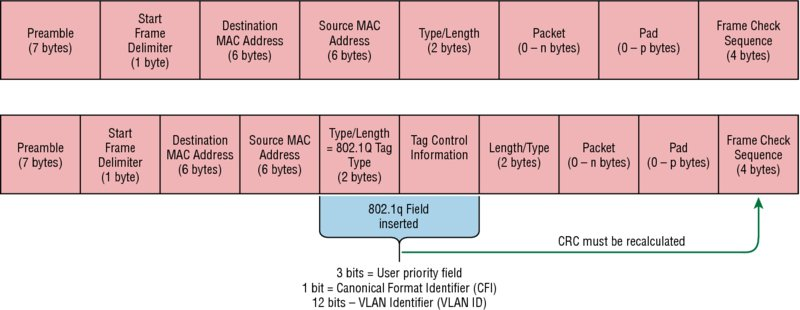
\includegraphics[width=.7\textwidth]{images/c11f007.jpg}
   \caption{IEEE 802.1q encapsulation with and without the 802.1q tag}
   \label{fig:802.1q-encapsulation}
\end{figure}


For the Cisco exam objectives, it's only the 12-bit VLAN ID that
matters. This field identifies the VLAN and can be 2 to the 12th, minus
2 for the 0 and 4,095 reserved VLANs, which means an 802.1q tagged frame
can carry information for 4,094 VLANs.

It works like this: You first designate each port that's going to be a
trunk with 802.1q encapsulation. The other ports must be assigned a
specific VLAN ID in order for them to communicate. VLAN 1 is the default
native VLAN, and when using 802.1q, all traffic for a native VLAN is
untagged. The ports that populate the same trunk create a group with
this native VLAN and each port gets tagged with an identification number
reflecting that. Again the default is VLAN 1. The native VLAN allows the
trunks to accept information that was received without any VLAN
identification or frame tag.

Most 2960 model switches only support the IEEE 802.1q trunking protocol,
but the 3560 will support both the ISL and IEEE methods, which you'll
see later in this chapter.

\begin{center}\rule{0.5\linewidth}{0.5pt}\end{center}

%\includegraphics{images/note.png}
The basic purpose of ISL and 802.1q
frame-tagging methods is to provide inter-switch VLAN communication.
Remember that any ISL or 802.1q frame tagging is removed if a frame is
forwarded out an access link -- tagging is used internally and across
trunk links only!

\begin{center}\rule{0.5\linewidth}{0.5pt}\end{center}



\section{Routing between VLANs}

Hosts in a VLAN live in their own broadcast domain and can communicate freely.
VLANs create network partitioning and traffic separation at layer~2 of the OSI, and as I said when I told you why we still need
routers, if you want hosts or any other IP-addressable device to communicate between VLANs, you must have a layer~3 device to provide routing.

For this, you can use a router that has an interface for each VLAN or a
router that supports ISL or 802.1q routing. The least expensive router
that supports ISL or 802.1q routing is the 2600 series router. You'd
have to buy that from a used-equipment reseller because they are
end-of-life, or EOL. I'd recommend at least a 2800 as a bare minimum,
but even that only supports 802.1q; Cisco is really moving away from
ISL, so you probably should only be using 802.1q anyway. Some 2800s may
support both ISL and 802.1q; I've just never seen it supported.

Anyway, as shown in
\protect\hyperlink{c11.xhtmlux5cux23figure11-8}{Figure 11.8}, if you had
two or three VLANs, you could get by with a router equipped with two or
three FastEthernet connections. And 10Base-T is okay for home study
purposes, and I mean only for your studies, but for anything else I'd
highly recommend Gigabit interfaces for real power under the hood!

What we see in \protect\hyperlink{c11.xhtmlux5cux23figure11-8}{Figure
11.8} is that each router interface is plugged into an access link. This
means that each of the routers' interface IP addresses would then become
the default gateway address for each host in each respective VLAN.

\begin{figure}
\centering
%\includegraphics{images/c11f008.jpg}
\caption{{\protect\hyperlink{c11.xhtmlux5cux23figureanchor11-8}{\textbf{FIGURE
11.8}} Router connecting three VLANs together for inter-VLAN
communication, one router interface for each VLAN}}
\end{figure}

If you have more VLANs available than router interfaces, you can
configure trunking on one FastEthernet interface or buy a layer~3
switch, like the old and now cheap 3560 or a higher-end switch like a
3850. You could even opt for a 6800 if you've got money to burn!

Instead of using a router interface for each VLAN, you can use one
FastEthernet interface and run ISL or 802.1q trunking.
\protect\hyperlink{c11.xhtmlux5cux23figure11-9}{Figure 11.9} shows how a
FastEthernet interface on a
router will look when
configured with ISL or 802.1q trunking. This allows all VLANs to
communicate through one interface. Cisco calls this a \emph{router-on-a-stick}
(ROAS).

\begin{figure}
\centering
%\includegraphics{images/c11f009.jpg}
\caption{{\protect\hyperlink{c11.xhtmlux5cux23figureanchor11-9}{\textbf{FIGURE
11.9}} Router-on-a-stick: single router interface connecting all three
VLANs together for inter-VLAN communication}}
\end{figure}

I really want to point out that this creates a potential bottleneck, as
well as a single point of failure, so your host/VLAN count is limited.
To how many? Well, that depends on your traffic level. To really make
things right, you'd be better off using a higher-end switch and routing
on the backplane. But if you just happen to have a router sitting
around, configuring this method is free, right?

\protect\hyperlink{c11.xhtmlux5cux23figure11-10}{Figure 11.10} shows how
we would create a router-on-a-stick using a router's physical interface
by creating logical interfaces -- one for each VLAN.

\begin{figure}
\centering
%\includegraphics{images/c11f010.jpg}
\caption{{\protect\hyperlink{c11.xhtmlux5cux23figureanchor11-10}{\textbf{FIGURE
11.10}} A router creates logical interfaces.}}
\end{figure}

Here we see one physical interface divided into multiple subinterfaces,
with one subnet assigned per VLAN, each subinterface being the default
gateway address for each VLAN/subnet. An encapsulation identifier must
be assigned to each subinterface to define the VLAN ID of that
subinterface. In the next section where I'll configure VLANs and
inter-VLAN routing, I'll configure our switched network with a router on
a stick and demonstrate this configuration for you.

But wait, there's still one more way to go about routing! Instead of
using an external router interface for each VLAN, or an external router
on a stick, we can configure logical interfaces on the backplane of the
layer~3 switch; this is called inter-VLAN routing (IVR), and it's
configured with a switched virtual interface (SVI).
\protect\hyperlink{c11.xhtmlux5cux23figure11-11}{Figure 11.11} shows how
hosts see these virtual interfaces.



\begin{figure}
\centering
%\includegraphics{images/c11f011.jpg}
\caption{{\protect\hyperlink{c11.xhtmlux5cux23figureanchor11-11}{\textbf{FIGURE
11.11}} With IVR, routing runs on the backplane of the switch, and it
appears to the hosts that a router is present.}}
\end{figure}

In \protect\hyperlink{c11.xhtmlux5cux23figure11-11}{Figure 11.11}, it
appears there's a router present, but there is no physical router
present as there was when we used router-on-a-stick. The IVR process
takes little effort and is easy to implement, which makes it very cool!
Plus, it's a lot more efficient for inter-VLAN routing than an external
router is. To implement IVR on a multilayer switch, we just need to
create logical interfaces in the switch configuration for each VLAN.
We'll configure this method in a minute, but first let's take our
existing switched network from Chapter 10, ``Layer 2 Switching,'' and
add some VLANs, then configure VLAN memberships and trunk links between
our switches.




\section{Configuring VLANs}

Now this may come as a surprise to you, but configuring VLANs is actually pretty easy.
It's just that figuring out which users you want
in each VLAN is not, and doing that can eat up a lot of your time! But
once you've decided on the number of VLANs you want to create and
established which users you want belonging to each one, it's time to
bring your first VLAN into the world.

To configure VLANs on a Cisco Catalyst switch, use the global config
\texttt{vlan} command. In the following example, I'm going to
demonstrate how to configure VLANs on the S1 switch by creating three
VLANs for three different departments -- again, remember that VLAN 1 is
the native and management VLAN by default:

\begin{cli}
S1(config)#vlan ?
 WORD        ISL VLAN IDs 1-4094
 access-map  Create vlan access-map or enter vlan access-map command mode
 dot1q       dot1q parameters
 filter      Apply a VLAN Map
 group       Create a vlan group
 internal    internal VLAN
S1(config)#vlan 2
S1(config-vlan)#name Sales
S1(config-vlan)#vlan 3
S1(config-vlan)#name Marketing
S1(config-vlan)#vlan 4
S1(config-vlan)#name Accounting
S1(config-vlan)#vlan 5
S1(config-vlan)#name Voice
S1(config-vlan)#^Z
S1#
\end{cli}

In this output, you can see that you can create VLANs from 1 to 4094.
But this is only mostly true.
As I said, VLANs can really only be created up to 1001, and you can't use, change, rename, or delete VLANs 1
or 1002 through 1005 because they're reserved.
The VLAN numbers above 1005 are called extended VLANs and won't be saved in the database unless your switch is set to what is called VLAN Trunking Protocol (VTP)
transparent mode.
You won't see these VLAN numbers used too often in production.
Here's an example of me attempting to set my S1 switch to VLAN 4000 when my switch is set to VTP server mode (the default VTP mode):

\begin{cli}
S1#config t
S1(config)#vlan 4000
S1(config-vlan)#^Z
% Failed to create VLANs 4000
Extended VLAN(s) not allowed in current VTP mode.
%Failed to commit extended VLAN(s) changes.
\end{cli}

After you create the VLANs that you want, you can use the
\texttt{show\ vlan} command to check them out. But notice that, by
default, all ports on the switch are in VLAN 1. To change the VLAN
associated with a port, you need to go to each interface and
specifically tell it which VLAN to be a part of.

\begin{center}\rule{0.5\linewidth}{0.5pt}\end{center}

%\includegraphics{images/note.png}
Remember that a created VLAN is unused
until it is assigned to a switch port or ports and that all ports are
always assigned in VLAN 1 unless set otherwise.

\begin{center}\rule{0.5\linewidth}{0.5pt}\end{center}

Once the VLANs are created, verify your configuration with the
\texttt{show\ vlan} command (\texttt{sh\ vlan} for short):

\begin{cli}
S1#sh vlan
VLAN Name              Status    Ports
---- ----------------- --------- -------------------------------
1    default           active    Fa0/1, Fa0/2, Fa0/3, Fa0/4
                                 Fa0/5, Fa0/6, Fa0/7, Fa0/8
                                 Fa0/9, Fa0/10, Fa0/11, Fa0/12
                                 Fa0/13, Fa0/14, Fa0/19, Fa0/20
                                 Fa0/21, Fa0/22, Fa0/23, Gi0/1
                                 Gi0/2
2    Sales             active
3    Marketing         active
4    Accounting        active
5    Voice             active
[output cut]
\end{cli}

This may seem repetitive, but it's important, and I want you to remember
it: You can't change, delete, or rename VLAN 1 because it's the default
VLAN and you just can't change that -- period. It's also the native VLAN
of all switches by default, and Cisco recommends that you use it as your
management VLAN. If you're worried about security issues, then change
it! Basically, any ports that aren't specifically assigned to a
different VLAN will be sent down to the native VLAN -- VLAN 1.

In the preceding S1 output, you can see that ports Fa0/1 through Fa0/14,
Fa0/19 through 23, and Gi0/1 and Gi0/2 uplinks are all in VLAN 1. But
where are ports 15 through 18? First, understand that the command
\texttt{show\ vlan} only displays access ports, so now that you know
what you're looking at with the \texttt{show\ vlan} command, where do
you think ports Fa15--18 are? That's right! They are trunked ports.
Cisco switches run a proprietary protocol called \emph{Dynamic Trunk
Protocol (DTP)}, and if there is a compatible switch connected, they
will start trunking automatically, which is precisely where my four
ports are. You have to use the \texttt{show\ interfaces\ trunk} command
to see your trunked ports like this:

\begin{cli}
S1# show interfaces trunk
Port        Mode             Encapsulation  Status        Native vlan
Fa0/15      desirable        n-isl          trunking      1
Fa0/16      desirable        n-isl          trunking      1
Fa0/17      desirable        n-isl          trunking      1
Fa0/18      desirable        n-isl          trunking      1

Port        Vlans allowed on trunk
Fa0/15      1-4094
Fa0/16      1-4094
Fa0/17      1-4094
Fa0/18      1-4094

[output cut]
\end{cli}

This output reveals that the VLANs from 1 to 4094 are allowed across the trunk by default.
Another helpful command, which is also part of the Cisco exam objectives, is the\texttt{show\ interfaces\ interface\ switchport} command:

\begin{cli}
S1#show interfaces fastEthernet 0/15 switchport
Name: Fa0/15
Switchport: Enabled
Administrative Mode: dynamic desirable
Operational Mode: trunk
Administrative Trunking Encapsulation: negotiate
Operational Trunking Encapsulation: isl
Negotiation of Trunking: On
Access Mode VLAN: 1 (default)
Trunking Native Mode VLAN: 1 (default)
Administrative Native VLAN tagging: enabled
Voice VLAN: none
[output cut]
\end{cli}

The highlighted output shows us the administrative mode of
\texttt{dynamic\ desirable}, that the port is a trunk port, and that DTP was used to negotiate the frame-tagging method of ISL.
It also predictably shows that the native VLAN is the default of 1.

Now that we can see the VLANs created, we can assign switch ports to specific ones.
Each port can be part of only one VLAN, with the exception of voice access ports.
Using trunking, you can make a port available to traffic from all VLANs.
I'll cover that next.

\subsection{Assigning switch ports to VLANs}

You configure a port to belong to a VLAN by assigning a membership mode
that specifies the kind of traffic the port carries plus the number of
VLANs it can belong to. You can also configure each port on a switch to
be in a specific VLAN (access port) by using the interface
\texttt{switchport} command. You can even configure multiple ports at
the same time with the \texttt{interface\ range} command.

In the next example, I'll configure interface Fa0/3 to VLAN 3. This is
the connection from the S3 switch to the host device:

\begin{cli}
S3#config t
S3(config)#int fa0/3
S3(config-if)#switchport ?
  access         Set access mode characteristics of the interface
  autostate      Include or exclude this port from vlan link up calculation
  backup         Set backup for the interface
  block          Disable forwarding of unknown uni/multi cast addresses
  host           Set port host
  mode           Set trunking mode of the interface
  nonegotiate    Device will not engage in negotiation protocol on this
                 interface
  port-security  Security related command
  priority       Set appliance 802.1p priority
  private-vlan   Set the private VLAN configuration
  protected      Configure an interface to be a protected port
  trunk          Set trunking characteristics of the interface
  voice          Voice appliance attributes voice
\end{cli}

Well now, what do we have here? There's some new stuff showing up in our
output now. We can see various commands -- some that I've already
covered, but no worries because I'm going to cover the \texttt{access},
\texttt{mode}, \texttt{nonegotiate}, and \texttt{trunk} commands very
soon. Let's start with setting an access port on S1, which is probably
the most widely used type of port you'll find on production switches
that have VLANs configured:

\begin{cli}
S3(config-if)#switchport mode ?
  access        Set trunking mode to ACCESS unconditionally
  dot1q-tunnel  set trunking mode to TUNNEL unconditionally
  dynamic       Set trunking mode to dynamically negotiate access or trunk mode
  private-vlan  Set private-vlan mode
  trunk         Set trunking mode to TRUNK unconditionally

S3(config-if)#switchport mode access
S3(config-if)#switchport access vlan 3
S3(config-if)#switchport voice vlan 5
\end{cli}

By starting with the \texttt{switchport\ mode\ access} command, you're
telling the switch that this is a nontrunking layer~2 port. You can then
assign a VLAN to the port with the \texttt{switchport\ access} command,
as well as configure the same port to be a member of a different type of
VLAN, called the \texttt{voice} VLAN. This allows you to connect a
laptop into a phone, and the phone into a single switch port. Remember,
you can choose many ports to configure simultaneously with the
\texttt{interface\ range} command.

Let's take a look at our VLANs now:

\begin{cli}
S3#show vlan
VLAN Name                       Status    Ports
---- ------------------------ --------- -------------------------------
1    default                   active     Fa0/4, Fa0/5, Fa0/6, Fa0/7
                                          Fa0/8, Fa0/9, Fa0/10, Fa0/11,
                                          Fa0/12, Fa0/13, Fa0/14, Fa0/19,
                                          Fa0/20, Fa0/21, Fa0/22, Fa0/23,
                                          Gi0/1, Gi0/2
2    Sales                     active
3    Marketing                 active    Fa0/3
5    Voice                     active    Fa0/3
\end{cli}

Notice that port Fa0/3 is now a member of VLAN 3 and VLAN 5 -- two different types of VLANs.
But, can you tell me where ports 1 and 2 are?
And why aren't they showing up in the output of \texttt{show\ vlan}?
That's right, because they are trunk ports!

We can also see this with the
\texttt{show\ interfaces\ interface\ switchport} command:

\begin{cli}
S3#sh int fa0/3 switchport
Name: Fa0/3
Switchport: Enabled
Administrative Mode: static access
Operational Mode: static access
Administrative Trunking Encapsulation: negotiate
Negotiation of Trunking: Off
Access Mode VLAN: 3 (Marketing)
Trunking Native Mode VLAN: 1 (default)
Administrative Native VLAN tagging: enabled
Voice VLAN: 5 (Voice)
\end{cli}

The highlighted output shows that Fa0/3 is an access port and a member
of VLAN 3 (Marketing), as well as a member of the Voice VLAN 5.

That's it. Well, sort of. If you plugged devices into each VLAN port,
they can only talk to other devices in the same VLAN. But as soon as you
learn a bit more about trunking, we're going to enable inter-VLAN
communication!



\subsection{Configuring trunk ports}

The 2960 switch only runs the IEEE 802.1q encapsulation method. To
configure trunking on a FastEthernet port, use the interface command
\texttt{switchport\ mode\ trunk}. It's a tad diff­erent on the 3560
switch.

The following switch output shows the trunk configuration on interfaces
Fa0/15--18 as set to \texttt{trunk}:

\begin{cli}
S1(config)#int range f0/15-18
S1(config-if-range)#switchport trunk encapsulation dot1q
S1(config-if-range)#switchport mode trunk
\end{cli}

If you have a switch that only runs the 802.1q encapsulation method,
then you wouldn't use the \texttt{encapsulation} command as I did in the
preceding output. Let's check out our trunk ports now:

\begin{cli}
S1(config-if-range)#do sh int f0/15 swi
Name: Fa0/15
Switchport: Enabled
Administrative Mode: trunk
Operational Mode: trunk
Administrative Trunking Encapsulation: dot1q
Operational Trunking Encapsulation: dot1q
Negotiation of Trunking: On
Access Mode VLAN: 1 (default)
Trunking Native Mode VLAN: 1 (default)
Administrative Native VLAN tagging: enabled
Voice VLAN: none
\end{cli}

Notice that port Fa0/15 is a trunk and running 802.1q.
Let's take another look:

\begin{cli}
S1(config-if-range)#do sh int trunk
Port        Mode             Encapsulation  Status        Native vlan
Fa0/15      on               802.1q         trunking      1
Fa0/16      on               802.1q         trunking      1
Fa0/17      on               802.1q         trunking      1
Fa0/18      on               802.1q         trunking      1
Port        Vlans allowed on trunk
Fa0/15      1-4094
Fa0/16      1-4094
Fa0/17      1-4094
Fa0/18      1-4094
\end{cli}

Take note of the fact that ports 15--18 are now in the trunk mode of on
and the encapsulation is now 802.1q instead of the negotiated ISL.
Here's a description of the different options available when configuring
a switch interface:

\texttt{switchport\ mode\ access} I discussed this in the previous
section, but this puts the interface (access port) into permanent
nontrunking mode and negotiates to convert the link into a nontrunk
link. The interface becomes a nontrunk interface regardless of whether
the neighboring interface is a trunk interface. The port would be a
dedicated layer~2 access port.

\texttt{switchport\ mode\ dynamic\ auto} This mode makes the interface
able to convert the link to a trunk link. The interface becomes a trunk
interface if the neighboring interface is set to trunk or desirable
mode. The default is \texttt{dynamic\ auto} on a lot of Cisco switches,
but that default trunk method is changing to \texttt{dynamic\ desirable}
on most new models.

\texttt{switchport\ mode\ dynamic\ desirable} This one makes the
interface actively attempt to convert the link to a trunk link. The
interface becomes a trunk interface if the neighboring interface is set
to \texttt{trunk}, \texttt{desirable}, or \texttt{auto} mode. I used to
see this mode as the default on some switches, but not any longer. This
is now the default switch port mode for all Ethernet interfaces on all
new Cisco switches.

\texttt{switchport\ mode\ trunk} Puts the interface into permanent
trunking mode and negotiates to convert the neighboring link into a
trunk link. The interface becomes a trunk interface even if the
neighboring interface isn't a trunk interface.

\texttt{switchport\ nonegotiate} Prevents the interface from generating
DTP frames. You can use this command only when the interface switchport
mode is access or trunk. You must manually configure the neighboring
interface as a trunk interface to establish a trunk link.

\begin{center}\rule{0.5\linewidth}{0.5pt}\end{center}

%\includegraphics{images/note.png}
Dynamic Trunking Protocol (DTP) is used
for negotiating trunking on a link between two devices as well as
negotiating the encapsulation type of either 802.1q or ISL. I use the
\texttt{nonegotiate} command when I want dedicated trunk ports; no
questions asked.

\begin{center}\rule{0.5\linewidth}{0.5pt}\end{center}

To disable trunking on an interface, use the \texttt{switchport\ mode\ access} command,
which sets the port back to a dedicated layer~2 access switch port.




\subsection{Defining the allowed VLANs on a trunk}

As I've mentioned, trunk ports send and receive information from all
VLANs by default, and if a frame is untagged, it's sent to the
management VLAN. Understand that this applies to the extended range
VLANs too.

But we can remove VLANs from the allowed list to prevent traffic from
certain VLANs from traversing a trunked link. I'll show you how you'd do
that, but first let me again demonstrate that all VLANs are allowed
across the trunk link by default:

\begin{verbatim}
S1# show interfaces trunk
[output cut]
Port        Vlans allowed on trunk
Fa0/15      1-4094
Fa0/16      1-4094
Fa0/17      1-4094
Fa0/18      1-4094
S1(config)#S1(config)#
S1(config-if)#S1(config-if)#
S1(config-if)#S1(config-if)#
[output cut]
Port        Vlans allowed on trunk
Fa0/15      4,6,12,15
Fa0/16      1-4094
Fa0/17      1-4094
Fa0/18      1-4094
\end{verbatim}

The preceding command affected the trunk link configured on S1 port
F0/15, causing it to permit all traffic sent and received for VLANs 4,
6, 12, and 15. You can try to remove VLAN 1 on a trunk link, but it will
still send and receive management like CDP, DTP, and VTP, so what's the
point?

To remove a range of VLANs, just use the hyphen:

\begin{verbatim}
S1(config-if)#switchport trunk allowed vlan remove 4-8
\end{verbatim}

If by chance someone has removed some VLANs from a trunk link and you
want to set the trunk back to default, just use this command:

\begin{verbatim}
S1(config-if)#switchport trunk allowed vlan all
\end{verbatim}

Next, I want to show you how to configure a native VLAN for a trunk
before we start routing between VLANs.

\subsubsection[Changing or Modifying the Trunk Native
VLAN]{\texorpdfstring{\protect\hypertarget{c11.xhtmlux5cux23c11-sec-13}{}{}Changing
or Modifying the Trunk Native
VLAN}{Changing or Modifying the Trunk Native VLAN}}

You can change the trunk port native VLAN from VLAN 1, which many people
do for security reasons. To change the native VLAN, use the following
command:

\begin{verbatim}
S1(config)#int f0/15
S1(config-if)#switchport trunk native vlan ?
  <1-4094>  VLAN ID of the native VLAN when this port is in trunking mode
\end{verbatim}

\begin{verbatim}
S1(config-if)#switchport trunk native vlan 4
1w6d: %CDP-4-NATIVE_VLAN_MISMATCH: Native VLAN mismatch discovered on FastEthernet0/15 (4), with S3 FastEthernet0/1 (1).
\end{verbatim}

So we've changed our native VLAN on our trunk link to 4, and by using
the\texttt{show\ running-config} command, I can see the configuration
under the trunk link:

\begin{verbatim}
S1#sh run int f0/15
Building configuration...
\end{verbatim}

\begin{verbatim}
Current configuration : 202 bytes
!
interface FastEthernet0/15
 description 1st connection to S3
 switchport trunk encapsulation dot1q
 switchport trunk native vlan 4
 switchport trunk allowed vlan 4,6,12,15
 switchport mode trunk
end
\end{verbatim}

\begin{verbatim}
S1#!
\end{verbatim}

Oops -- wait a minute! You didn't think it would be this easy and would
just start working, did you? Of course not! Here's the rub: If all
switches don't have the same native VLAN configured on the given trunk
links, then we'll start to receive this error, which happened
immediately after I entered the command:

\begin{verbatim}
1w6d: %CDP-4-NATIVE_VLAN_MISMATCH: Native VLAN mismatch discovered
on FastEthernet0/15 (4), with S3 FastEthernet0/1 (1).
\end{verbatim}

Actually, this is a good, noncryptic error, so either we can go to the
other end of our trunk link(s) and change the native VLAN or we set the
native VLAN back to the default to fix it. Here's how we'd do that:

\begin{verbatim}
S1(config-if)#no switchport trunk native vlan
1w6d: %SPANTREE-2-UNBLOCK_CONSIST_PORT: Unblocking FastEthernet0/15
on VLAN0004. Port consistency restored.
\end{verbatim}

Now our trunk link is
using the default VLAN 1 as the native VLAN. Just remember that all
switches on a given trunk must use the same native VLAN or you'll have
some serious management problems. These issues won't affect user data,
just management traffic between switches. Now, let's mix it up by
connecting a router into our switched network and configure inter-VLAN
communication.

\subsubsection{Configuring inter-VLAN routing}

By default, only hosts that are members of the same VLAN can
communicate. To change this and allow inter-VLAN communication, you need
a router or a layer~3 switch. I'm going to start with the router
approach.

To support ISL or 802.1q routing on a FastEthernet interface, the
router's interface is divided into logical interfaces -- one for each
VLAN -- as was shown in
\protect\hyperlink{c11.xhtmlux5cux23figure11-10}{Figure 11.10}. These
are called \emph{subinterfaces}. From a FastEthernet or Gigabit
interface, you can set the interface to trunk with the
\texttt{encapsulation} command:

\begin{verbatim}
ISR#config t
ISR(config)#int f0/0.1
ISR(config-subif)#encapsulation ?
  dot1Q  IEEE 802.1Q Virtual LAN
ISR(config-subif)#encapsulation dot1Q ?
  <1-4094>  IEEE 802.1Q VLAN ID
\end{verbatim}

Notice that my 2811 router (named ISR) only supports 802.1q. We'd need
an older-model router to run the ISL encapsulation, but why bother?

The subinterface number is only locally significant, so it doesn't
matter which subinterface numbers are configured on the router. Most of
the time, I'll configure a subinterface with the same number as the VLAN
I want to route. It's easy to remember that way since the subinterface
number is used only for administrative purposes.

It's really important that you understand that each VLAN is actually a
separate subnet. True, I know -- they don't \emph{have} to be. But it
really is a good idea to configure your VLANs as separate subnets, so
just do that. Before we move on, I want to define \emph{upstream
routing}. This is a term used to define the router-on-a-stick. This
router will provide inter-VLAN routing, but it can also be used to
forward traffic upstream from the switched network to other parts of the
corporate network or Internet.

Now, I need to make sure you're fully prepared to configure inter-VLAN
routing as well as determine the IP addresses of hosts connected in a
switched VLAN environment. And as always, it's also a good idea to be
able to fix any problems that may arise. To set you up for success, let
me give you few examples.

First, start by looking at
\protect\hyperlink{c11.xhtmlux5cux23figure11-12}{Figure 11.12} and read
the router and switch configuration within it. By this point in the
book, you should be able to determine the IP address, masks, and default
gateways of each of the hosts in the VLANs.



\begin{figure}
\centering
%\includegraphics{images/c11f012.jpg}
\caption{{\protect\hyperlink{c11.xhtmlux5cux23figureanchor11-12}{\textbf{FIGURE
11.12}} Configuring inter-VLAN example 1}}
\end{figure}

The next step is to figure out which subnets are being used. By looking
at the router configuration in the figure, you can see that we're using
192.168.10.0/28 for VLAN1, 192.168.1.64/26 with VLAN 2, and
192.168.1.128/27 for VLAN 10.

By looking at the switch configuration, you can see that ports 2 and 3
are in VLAN 2 and port 4 is in VLAN 10. This means that Host A and Host
B are in VLAN 2 and Host C is in VLAN 10.

But wait -- what's that IP address doing there under the physical
interface? Can we even do that? Sure we can! If we place an IP address
under the physical interface, the result is that frames sent from the IP
address would be untagged. So what VLAN would those frames be a member
of? By default, they would belong to VLAN 1, our management VLAN. This
means the address 192.168.10.1 /28 is my native VLAN IP address for this
switch.

Here's what the hosts' IP addresses should be:

\begin{enumerate}
\tightlist
\item
  \textbf{Host A:} 192.168.1.66, 255.255.255.192, default gateway
  192.168.1.65
\item
  \textbf{Host B:} 192.168.1.67, 255.255.255.192, default gateway
  192.168.1.65
\item
  \textbf{Host C:} 192.168.1.130, 255.255.255.224, default gateway
  192.168.1.129
\end{enumerate}

The hosts could be any address in the range -- I just chose the first
available IP address after the default gateway address. That wasn't so
hard, was it?

Now, again using \protect\hyperlink{c11.xhtmlux5cux23figure11-12}{Figure
11.12}, let's go through the commands necessary to configure switch port
1 so it will establish a link with the router and provide inter-VLAN
communication using the IEEE version for encapsulation. Keep in mind
that the commands can vary slightly depending on what type of switch
you're dealing with.

For a 2960 switch, use the following:

\begin{verbatim}
2960#config t
2960(config)#interface fa0/1
2960(config-if)#switchport mode trunk
\end{verbatim}

That's it! As you
already know, the 2960 switch can only run the 802.1q encapsulation, so
there's no need to specify it. You can't anyway. For a 3560, it's
basically the same, but because it can run ISL and 802.1q, you have to
specify the trunking encapsulation protocol you're going to use.

\begin{center}\rule{0.5\linewidth}{0.5pt}\end{center}

%\includegraphics{images/note.png}
Remember that when you create a trunked
link, all VLANs are allowed to pass data by default.

\begin{center}\rule{0.5\linewidth}{0.5pt}\end{center}

Let's take a look at
\protect\hyperlink{c11.xhtmlux5cux23figure11-13}{Figure 11.13} and see
what we can determine. This figure shows three VLANs, with two hosts in
each of them. The router in
\protect\hyperlink{c11.xhtmlux5cux23figure11-13}{Figure 11.13} is
connected to the Fa0/1 switch port, and VLAN 4 is configured on port
F0/6.

When looking at this diagram, keep in mind that these three factors are
what Cisco expects you to know:

\begin{enumerate}
\tightlist
\item
  The router is connected to the switch using subinterfaces.
\item
  The switch port connecting to the router is a trunk port.
\item
  The switch ports connecting to the clients and the hub are access
  ports, not trunk ports.
\end{enumerate}

\begin{figure}
\centering
%\includegraphics{images/c11f013.jpg}
\caption{{\protect\hyperlink{c11.xhtmlux5cux23figureanchor11-13}{\textbf{FIGURE
11.13}} Inter-VLAN example 2}}
\end{figure}

The configuration of the switch would look something like this:

\begin{verbatim}
2960#config t
2960(config)#int f0/1
2960(config-if)#switchport mode trunk
2960(config-if)#int f0/2
2960(config-if)#switchport access vlan 2
2960(config-if)#int f0/3
2960(config-if)#switchport access vlan 2
2960(config-if)#int f0/4
2960(config-if)#switchport access vlan 3
2960(config-if)#int f0/5
2960(config-if)#switchport access vlan 3
2960(config-if)#int f0/6
2960(config-if)#switchport access vlan 4
\end{verbatim}

Before we configure the router, we need to design our logical network:

\begin{enumerate}
\tightlist
\item
  \textbf{VLAN 1:} 192.168.10.0/28
\item
  \textbf{VLAN 2:} 192.168.10.16/28
\item
  \textbf{VLAN 3:} 192.168.10.32/28
\item
  \textbf{VLAN 4:} 192.168.10.48/28
\end{enumerate}

The configuration of the router would then look like this:

\begin{verbatim}
ISR#config t
ISR(config)#int fa0/0
ISR(config-if)#ip address 192.168.10.1 255.255.255.240
ISR(config-if)#no shutdown
ISR(config-if)#int f0/0.2
ISR(config-subif)#encapsulation dot1q 2
ISR(config-subif)#ip address 192.168.10.17 255.255.255.240
ISR(config-subif)#int f0/0.3
ISR(config-subif)#encapsulation dot1q 3
ISR(config-subif)#ip address 192.168.10.33 255.255.255.240
ISR(config-subif)#int f0/0.4
ISR(config-subif)#encapsulation dot1q 4
ISR(config-subif)#ip address 192.168.10.49 255.255.255.240
\end{verbatim}

Notice I didn't tag VLAN 1. Even though I could have created a
subinterface and tagged VLAN 1, it's not necessary with 802.1q because
untagged frames are members of the native VLAN.

The hosts in each VLAN would be assigned an address from their subnet
range, and the default gateway would be the IP address assigned to the
router's subinterface in that VLAN.

Now, let's take a look at another figure and see if you can determine
the switch and router configurations without looking at the answer -- no
cheating! \protect\hyperlink{c11.xhtmlux5cux23figure11-14}{Figure 11.14}
shows a router connected to a 2960 switch with two VLANs. One host in
each VLAN is assigned
an IP address. What
would your router and switch configurations be based on these IP
addresses?

\begin{figure}
\centering
%\includegraphics{images/c11f014.jpg}
\caption{{\protect\hyperlink{c11.xhtmlux5cux23figureanchor11-14}{\textbf{FIGURE
11.14}} Inter-VLAN example 3}}
\end{figure}

Since the hosts don't list a subnet mask, you have to look for the
number of hosts used in each VLAN to figure out the block size. VLAN 2
has 85 hosts and VLAN 3 has 115 hosts. Each of these will fit in a block
size of 128, which is a /25 mask, or 255.255.255.128.

You should know by now that the subnets are 0 and 128; the 0 subnet
(VLAN 2) has a host range of 1--126, and the 128 subnet (VLAN 3) has a
range of 129--254. You can almost be fooled since Host A has an IP
address of 126, which makes it \emph{almost} seem that Host A and B are
in the same subnet. But they're not, and you're way too smart by now to
be fooled by this one!

Here is the switch configuration:

\begin{verbatim}
2960#config t
2960(config)#int f0/1
2960(config-if)#switchport mode trunk
2960(config-if)#int f0/2
2960(config-if)#switchport access vlan 2
2960(config-if)#int f0/3
2960(config-if)#switchport access vlan 3
\end{verbatim}

Here is the router configuration:

\begin{verbatim}
ISR#config t
ISR(config) # int f0/0
ISR(config-if)#ip address 192.168.10.1 255.255.255.0
ISR(config-if)#no shutdown
ISR(config-if)#int f0/0.2
ISR(config-subif)#encapsulation dot1q 2
ISR(config-subif)#ip address 172.16.10.1 255.255.255.128
ISR(config-subif)#int f0/0.3
ISR(config-subif)#encapsulation dot1q 3
ISR(config-subif)#ip address 172.16.10.254 255.255.255.128
\end{verbatim}

I used the first address in the host range for VLAN 2 and the last
address in the range for VLAN 3, but any address in the range would
work. You would just have to configure the host's default gateway to
whatever you make the router's address. Also, I used a different subnet
for my physical interface, which is my management VLAN router's address.

Now, before we go on to the next example, I need to make sure you know
how to set the IP address on the switch. Since VLAN 1 is typically the
administrative VLAN, we'll use an IP address from out of that pool of
addresses. Here's how to set the IP address of the switch (not nagging,
but you really should already know this!):

\begin{verbatim}
2960#config t
2960(config)#int vlan 1
2960(config-if)#ip address 192.168.10.2 255.255.255.0
2960(config-if)#no shutdown
2960(config-if)#exit
2960(config)#ip default-gateway 192.168.10.1
\end{verbatim}

Yes, you have to execute a \texttt{no\ shutdown} on the VLAN interface
and set the \texttt{ip\ default-gateway} address to the router.

One more example, and then we'll move on to IVR using a multilayer
switch -- another important subject that you definitely don't want to
miss! In \protect\hyperlink{c11.xhtmlux5cux23figure11-15}{Figure 11.15}
there are two VLANs, plus the management VLAN 1. By looking at the
router configuration, what's the IP address, subnet mask, and default
gateway of Host A? Use the last IP address in the range for Host A's
address.

If you really look carefully at the router configuration (the hostname
in this configuration is just Router), there's a simple and quick
answer. All subnets are using a /28, which is a 255.255.255.240 mask.
This is a block size of 16. The router's address for VLAN 2 is in subnet
128. The next subnet is 144, so the broadcast address of VLAN 2 is 143
and the valid host range is 129--142. So the host address would be this:

\begin{enumerate}
\tightlist
\item
  \textbf{IP address:} 192.168.10.142
\item
  \textbf{Mask:} 255.255.255.240
\item
  \textbf{Default gateway:} 192.168.10.129
\end{enumerate}



\begin{figure}
\centering
%\includegraphics{images/c11f015.jpg}
\caption{{\protect\hyperlink{c11.xhtmlux5cux23figureanchor11-15}{\textbf{FIGURE
11.15}} Inter-VLAN example 4}}
\end{figure}

This section was probably the hardest part of this entire book, and I
honestly created the simplest configuration you can possibly get away
with using to help you through it!

I'll use \protect\hyperlink{c11.xhtmlux5cux23figure11-16}{Figure 11.16}
to demonstrate configuring inter-VLAN routing (IVR) with a multi­layer
switch, which is often referred to as a switched virtual interface
(SVI). I'm going to use the same network that I used to discuss a
multilayer switch back in
\protect\hyperlink{c11.xhtmlux5cux23figure11-11}{Figure 11.11}, and I'll
use this IP address scheme: 192.168.\emph{x}.0/24, where \emph{x}
represents the VLAN subnet. In my example this will be the same as the
VLAN number.

\begin{figure}
\centering
%\includegraphics{images/c11f016.jpg}
\caption{{\protect\hyperlink{c11.xhtmlux5cux23figureanchor11-16}{\textbf{FIGURE
11.16}} Inter-VLAN routing with a multilayer switch}}
\end{figure}

The hosts are already configured with the IP address, subnet mask, and
default gateway address using the first address in the range. Now I just
need to configure the routing on the switch, which is pretty simple
actually:

\begin{verbatim}
S1(config)#ip routing
S1(config)#int vlan 10
S1(config-if)#ip address 192.168.10.1 255.255.255.0
S1(config-if)#int vlan 20
S1(config-if)#ip address 192.168.20.1 255.255.255.0
\end{verbatim}

And that's it! Enable IP routing and create one logical interface for
each VLAN using the \texttt{interface\ vlan\ number} command and voilà!
You've now accomplished making inter-VLAN routing work on the backplane
of the switch!

\section{Summary}

In this chapter, I introduced you to the world of virtual LANs and
described how Cisco switches can use them. We talked about how VLANs
break up broadcast domains in a switched internetwork -- a very
important, necessary thing because layer~2 switches only break up
collision domains, and by default, all switches make up one large
broadcast domain. I also described access links to you, and we went over
how trunked VLANs work across a FastEthernet or faster link.

Trunking is a crucial technology to understand really well when you're
dealing with a network populated by multiple switches that are running
several VLANs.

You were also presented with some key troubleshooting and configuration
examples for access and trunk ports, configuring trunking options, and a
huge section on IVR.

\section{Exam Essentials}

\textbf{Understand the term}\emph{frame tagging}. \emph{Frame tagging}
refers to VLAN identification; this is what switches use to keep track
of all those frames as they're traversing a switch fabric. It's how
switches identify which frames belong to which VLANs.

\textbf{Understand the 802.1q VLAN identification method.} This is a
nonproprietary IEEE method of frame tagging. If you're trunking between
a Cisco switched link and a different brand of switch, you have to use
802.1q for the trunk to work.

\textbf{Remember how to set a trunk port on a 2960 switch.} To set a
port to trunking on a 2960, use the \texttt{switchport\ mode\ trunk}
command.

\textbf{Remember to check a switch port's VLAN assignment when plugging
in a new host.} If you plug a new host into a switch, then you must
verify the VLAN membership of that port. If the membership is different
than what is needed for that host, the host will not be able to reach
the needed network services, such as a workgroup server or printer.

\textbf{Remember how to create a Cisco router-on-a-stick to provide
inter-VLAN communication.} You can use a Cisco FastEthernet or Gigabit
Ethernet interface to provide inter-VLAN routing. The switch port
connected to the router must be a trunk port; then you must create
virtual interfaces
(subinterfaces) on the router port for each VLAN connecting to it. The
hosts in each VLAN will use this subinterface address as their default
gateway address.

\textbf{Remember how to provide inter-VLAN routing with a layer~3
switch.} You can use a layer~3 (multilayer) switch to provide IVR just
as with a router-on-a-stick, but using a layer~3 switch is more
efficient and faster. First you start the routing process with the
command\texttt{ip\ routing}, then create a virtual interface for each
VLAN using the command \texttt{interface\ vlan\ vlan}, and then apply
the IP address for that VLAN under that logical interface.

\section{Written lab}

In this section, you'll complete the following lab to make sure you've
got the information and concepts contained within them fully dialed in:

Lab 11.1: VLANs

You can find the answers to this lab in Appendix A, ``Answers to Written
Labs.''

Write the answers to the following questions:

\begin{enumerate}
\tightlist
\item
  True/False: To provide IVR with a layer~3 switch, you place an IP
  address on each interface of the switch.
\item
  What protocol will stop loops in a layer~2 switched network?
\item
  VLANs break up \_\_\_\_\_\_\_\_\_\_\_ domains in a layer~2 switched
  network.
\item
  Which VLAN numbers are reserved by default?
\item
  If you have a switch that provides both ISL and 802.1q frame tagging,
  what command under the trunk interface will make the trunk use 802.1q?
\item
  What does trunking provide?
\item
  How many VLANs can you create on an IOS switch by default?
\item
  True/False: The 802.1q encapsulation is removed from the frame if the
  frame is forwarded out an access link.
\item
  What type of link on a switch is a member of only one VLAN?
\item
  You want to change from the default of VLAN 1 to VLAN 4 for untagged
  traffic. What command will you use?
\end{enumerate}




\section{Hands-on labs}

In these labs, you will use three switches and a router.
To perform the last lab, you'll need a layer~3 switch.

\begin{enumerate}
\tightlist
\item
  Lab 11.1: Configuring and Verifying VLANs
\item
  Lab 11.2: Configuring and Verifying Trunk Links
\item
  Lab 11.3:
  Configuring Router on a Stick Routing
\item
  Lab 11.4: Configuring IVR with a Layer 3 Switch
\end{enumerate}

In these labs, I'll use the following layout:

\begin{figure}
\centering
%\includegraphics{images/c11f017.jpg}
\caption{}
\end{figure}

\subsection{Configuring and verifying VLANs}

This lab will have you configure VLANs from global configuration mode
and then verify the VLANs.

\begin{enumerate}
\item
  Configure two VLANs on each switch, VLAN 10 and VLAN 20.

\begin{verbatim}
S1(config)#vlan 10
S1(config-vlan)#vlan 20
\end{verbatim}

\begin{verbatim}
S2(config)#vlan 10
S2(config-vlan)#vlan 20
\end{verbatim}

\begin{verbatim}
S3(config)#vlan 10
S3(config-vlan)#vlan 20
\end{verbatim}
\item
  Use the \texttt{show\ vlan} and \texttt{show\ vlan\ brief} commands to
  verify your VLANs. Notice that all interfaces are in VLAN 1 by
  default.

\begin{verbatim}
S1#sh vlan
S1#sh vlan brief
\end{verbatim}
\end{enumerate}

\subsection{Configuring and verifying trunk links}

This lab will have you configure trunk links and then verify them.

\begin{enumerate}
\item
  Connect to each
  switch and configure trunking on all switch links. If you are using a
  switch that supports both 802.1q and ISL frame tagging, then use the
  encapsulation command; if not, then skip that command.

\begin{verbatim}
S1#config t
S1(config)#interface fa0/15
S1(config-if)#switchport trunk encapsulation ?
  dot1q  Interface uses only 802.1q trunking encapsulation when trunking
  isl    Interface uses only ISL trunking encapsulation when trunking
  negotiate   Device will negotiate trunking encapsulation with peer on interface
\end{verbatim}

  Again, if you typed the previous and received an error, then your
  switch does not support both encapsulation methods:

\begin{verbatim}
S1 (config-if)#switchport trunk encapsulation dot1q
S1 (config-if)#switchport mode trunk
S1 (config-if)#interface fa0/16
S1 (config-if)#switchport trunk encapsulation dot1q
S1 (config-if)#switchport mode trunk
S1 (config-if)#interface fa0/17
S1 (config-if)#switchport trunk encapsulation dot1q
S1 (config-if)#switchport mode trunk
S1 (config-f)#interface fa0/18
S1 (config-if)#switchport trunk encapsulation dot1q
S1 (config-if)#switchport mode trunk
\end{verbatim}
\item
  Configure the trunk links on your other switches.
\item
  On each switch, verify your trunk ports with the
  \texttt{show\ interface\ trunk} command:

\begin{verbatim}
S1#show interface trunk
\end{verbatim}
\item
  Verify the switchport configuration with the following:

\begin{verbatim}
S1#show interface interface switchport
\end{verbatim}
\end{enumerate}

The second \texttt{interface}in the command is a variable, such as
Fa0/15.

\subsection{Configuring router-on-a-stick routing}

In this lab, you'll use the router connected to port F0/8 of switch S1
to configure a router-on-a-stick.

\begin{enumerate}
\item
  Configure the F0/0 of the router with two subinterfaces to provide
  inter-VLAN routing using 802.1q encapsulation. Use 172.16.10.0/24 for
  your management VLAN, 10.10.10.0/24 for VLAN 10, and 20.20.20.0/24 for
  VLAN 20.

\begin{verbatim}
Router#config t
Router (config)#int f0/0
Router (config-if)#ip address 172.16.10.1 255.255.255.0
Router (config-if)#interface f0/0.10
Router (config-subif)#encapsulation dot1q 10
Router (config-subif)#ip address 10.10.10.1 255.255.255.0
Router (config-subif)#interface f0/0.20
Router (config-subif)#encapsulation dot1q 20
Router (config-subif)#ip address 20.20.20.1 255.255.255.0
\end{verbatim}
\item
  Verify the configuration with the \texttt{show\ running-config}
  command.
\item
  Configure trunking on interface F0/8 of the S1 switch connecting to
  your router.
\item
  Verify that your VLANs are still configured on your switches with the
  \texttt{sh\ vlan} command.
\item
  Configure your hosts to be in VLAN 10 and VLAN 20 with the
  \texttt{switchport\ access\ vlan\ x} command.
\item
  Ping from your PC to the router's subinterface configured for your
  VLAN.
\item
  Ping from your PC to your PC in the other VLAN. You are now routing
  through the router!
\end{enumerate}

\subsection{Configuring IVR with a layer~3 switch}

In this lab, you will disable the router and use the S1 switch to
provide inter-VLAN routing by creating SVI's.

\begin{enumerate}
\item
  Connect to the S1 switch and make interface F0/8 an access port, which
  will make the router stop providing inter-VLAN routing.
\item
  Enable IP routing on the S1 switch.

\begin{verbatim}
S1(config)#ip routing
\end{verbatim}
\item
  Create two new interfaces on the S1 switch to provide IVR.

\begin{verbatim}
S1(config)#interface vlan 10
S1(config-if)#ip address 10.10.10.1 255.255.255.0
S1(config-if)#interface vlan 20
S1(config-if)#ip address 20.20.20.1 255.255.255.0
\end{verbatim}
\item
  Clear the ARP cache on the switch and hosts.

\begin{verbatim}
S1#clear arp
\end{verbatim}
\item
  Ping from your PC to the router's subinterface configured for your
  VLAN.
\item
  Ping from your PC to your PC in the other VLAN. You are now routing
  through the S1 switch!
\end{enumerate}




\section{Review questions}

You can find the answers to these questions in Appendix B, ``Answers to Review Questions.''

\begin{enumerate}
\item
  Which of the following statements is true with regard to VLANs?

  \begin{enumerate}
  \tightlist
  \item
    VLANs greatly reduce network security.
  \item
    VLANs increase the number of collision domains while decreasing
    their size.
  \item
    VLANs decrease the number of broadcast domains while decreasing
    their size.
  \item
    Network adds, moves, and changes are achieved with ease by just
    configuring a port into the appropriate VLAN.
  \end{enumerate}
\item
  Write the command that must be present for this layer~3 switch to
  provide inter-VLAN routing between the two VLANs created with these
  commands:

\begin{verbatim}
S1(config)#int vlan 10
S1(config-if)#ip address 192.168.10.1 255.255.255.0
S1(config-if)#int vlan 20
S1(config-if)#ip address 192.168.20.1 255.255.255.0
\end{verbatim}
\item
  In the following diagram, how must the port on each end of the line be
  configured to carry traffic between the four hosts?

  \begin{figure}
  \centering
  %\includegraphics{images/c11f018.jpg}
  \caption{}
  \end{figure}

  \begin{enumerate}
  \tightlist
  \item
     Access port
  \item
    10 GB
  \item
    Trunk
  \item
    Spanning
  \end{enumerate}
\item
  What is the only type of \emph{second} VLAN of which an access port
  can be a member?

  \begin{enumerate}
  \tightlist
  \item
    Secondary
  \item
    Voice
  \item
    Primary
  \item
    Trunk
  \end{enumerate}
\item
  In the following configuration, what command is missing in the
  creation of the VLAN interface?

\begin{verbatim}
2960#config t
2960(config)#int vlan 1
2960(config-if)#ip address 192.168.10.2 255.255.255.0
2960(config-if)#exit
2960(config)#ip default-gateway 192.168.10.1
\end{verbatim}

  \begin{enumerate}
  \tightlist
  \item
    \texttt{no\ shutdown} under int vlan 1
  \item
    \texttt{encapsulation\ dot1q\ 1} under int vlan 1
  \item
    \texttt{switchport\ access\ vlan\ 1}
  \item
    \texttt{passive-interface}
  \end{enumerate}
\item
  Which of the following statements is true with regard to ISL and
  802.1q?

  \begin{enumerate}
  \tightlist
  \item
    802.1q encapsulates the frame with control information; ISL inserts
    an ISL field along with tag control information.
  \item
    802.1q is Cisco proprietary.
  \item
    ISL encapsulates the frame with control information; 802.1q inserts
    an 802.1q field along with tag control information.
  \item
    ISL is a standard.
  \end{enumerate}
\item
  What concept is depicted in the diagram?

  \begin{figure}
  \centering
  %\includegraphics{images/c11f019.jpg}
  \caption{}
  \end{figure}

  \begin{enumerate}
  \tightlist
  \item
     Multiprotocol
    routing
  \item
    Passive interface
  \item
    Gateway redundancy
  \item
    Router-on-a-stick
  \end{enumerate}
\item
  Write the command that places an interface into VLAN 2. Write only the
  command and not the prompt.
\item
  Write the command that generated the following output:

\begin{verbatim}
VLAN Name                       Status    Ports
---- ------------------------- --------- ------------------------
1    default                    active   Fa0/1, Fa0/2, Fa0/3, Fa0/4
                                         Fa0/5, Fa0/6, Fa0/7, Fa0/8
                                       Fa0/9, Fa0/10, Fa0/11, Fa0/12
                                      Fa0/13, Fa0/14, Fa0/19, Fa0/20
                                      Fa0/21, Fa0/22, Fa0/23, Gi0/1
                                          Gi0/2
2    Sales                      active
3    Marketing                  active
4    Accounting                 active
[output cut]
\end{verbatim}
\item
  In the configuration and diagram shown, what command is missing to
  enable inter-VLAN routing between VLAN 2 and VLAN 3?

  \begin{figure}
  \centering
  %\includegraphics{images/c11f020.jpg}
  \caption{}
  \end{figure}

  \begin{enumerate}
  \tightlist
  \item
    \texttt{encapsulation\ dot1q\ 3} under int f0/0.2
  \item
    \texttt{encapsulation\ dot1q\ 2} under int f0/0.2
  \item
    \texttt{no\ shutdown} under int f0/0.2
  \item
    \texttt{no\ shutdown} under int f0/0.3
  \end{enumerate}
\item
   Based on the
  configuration shown here, what statement is true?

\begin{verbatim}
S1(config)#ip routing
S1(config)#int vlan 10
S1(config-if)#ip address 192.168.10.1 255.255.255.0
S1(config-if)#int vlan 20
S1(config-if)#ip address 192.168.20.1 255.255.255.0
\end{verbatim}

  \begin{enumerate}
  \tightlist
  \item
    This is a multilayer switch.
  \item
    The two VLANs are in the same subnet.
  \item
    Encapsulation must be configured.
  \item
    VLAN 10 is the management VLAN.
  \end{enumerate}
\item
  What is true of the output shown here?

\begin{verbatim}
S1#sh vlan
VLAN Name                    Status    Ports
---- ---------------------- --------- -------------------------------
1    default                 active    Fa0/1, Fa0/2, Fa0/3, Fa0/4
                                       Fa0/5, Fa0/6, Fa0/7, Fa0/8
                                       Fa0/9, Fa0/10, Fa0/11, Fa0/12
                                       Fa0/13, Fa0/14, Fa0/19, Fa0/20,
                                       Fa0/22, Fa0/23, Gi0/1, Gi0/2
2    Sales                   active
3    Marketing               active    Fa0/21
4    Accounting              active
[output cut]
\end{verbatim}

  \begin{enumerate}
  \tightlist
  \item
    Interface F0/15 is a trunk port.
  \item
    Interface F0/17 is an access port.
  \item
    Interface F0/21 is a trunk port.
  \item
    VLAN 1 was populated manually.
  \end{enumerate}
\item
  802.1q untagged frames are members of the \_\_\_\_\_\_\_\_\_\_ VLAN.

  \begin{enumerate}
  \tightlist
  \item
    Auxiliary
  \item
    Voice
  \item
    Native
  \item
    Private
  \end{enumerate}
\item
   Write the command
  that generated the following output. Write only the command and not
  the prompt:

\begin{verbatim}
Name: Fa0/15
Switchport: Enabled
Administrative Mode: dynamic desirable
Operational Mode: trunk
Administrative Trunking Encapsulation: negotiate
Operational Trunking Encapsulation: isl
Negotiation of Trunking: On
Access Mode VLAN: 1 (default)
Trunking Native Mode VLAN: 1 (default)
Administrative Native VLAN tagging: enabled
Voice VLAN: none
[output cut]
\end{verbatim}
\item
  In the switch output of question 12, how many broadcast domains are
  shown?

  \begin{enumerate}
  \tightlist
  \item
    1
  \item
    2
  \item
    4
  \item
    1001
  \end{enumerate}
\item
  In the diagram, what should be the default gateway address of Host B?

  \begin{figure}
  \centering
  %\includegraphics{images/c11f021.jpg}
  \caption{}
  \end{figure}

  \begin{enumerate}
  \tightlist
  \item
    192.168.10.1
  \item
    192.168.1.65
  \item
    192.168.1.129
  \item
    192.168.1.2
  \end{enumerate}
\item
   What is the
  purpose of frame tagging in virtual LAN (VLAN) configurations?

  \begin{enumerate}
  \tightlist
  \item
    Inter-VLAN routing
  \item
    Encryption of network packets
  \item
    Frame identification over trunk links
  \item
    Frame identification over access links
  \end{enumerate}
\item
  Write the command to create VLAN 2 on a layer~2 switch. Write only the
  command and not the prompt.
\item
  Which statement is true regarding 802.1q frame tagging?

  \begin{enumerate}
  \tightlist
  \item
    802.1q adds a 26-byte trailer and 4-byte header.
  \item
    802.1q uses a native VLAN.
  \item
    The original Ethernet frame is not modified.
  \item
    802.1q only works with Cisco switches.
  \end{enumerate}
\item
  Write the command that prevents an interface from generating DTP
  frames. Write only the command and not the prompt.
\end{enumerate}



